\documentclass[]{article}

\usepackage[utf8]{inputenc}
\usepackage[usenames,dvipsnames]{xcolor}
\usepackage{fullpage}
\usepackage[upright]{fourier}
\usepackage{tkz-graph}
\usepackage{color}
\usetikzlibrary{arrows}

\usepackage[paperheight=2.1in,paperwidth=2.7in,margin=0in]{geometry}
\definecolor{color1}{RGB}{251,180,174}
\definecolor{color2}{RGB}{179,205,227}
\definecolor{color3}{RGB}{204,235,197}
\definecolor{color4}{RGB}{222,203,227}

\begin{document}
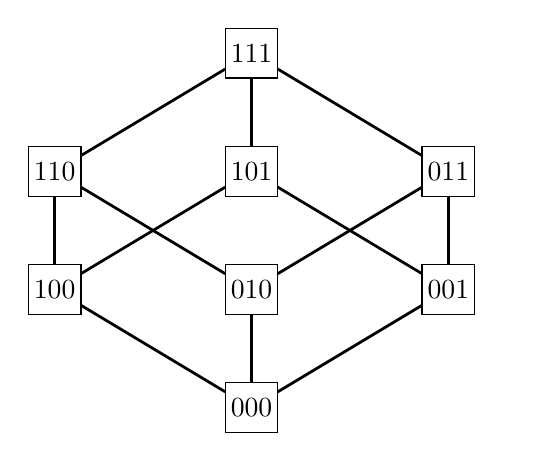
\begin{tikzpicture}
  \SetVertexNormal[Shape     = rectangle,
                   FillColor = white,
                  LineWidth  = 1pt]
  \SetUpEdge[lw         = 1pt,
             color      = black,
             labelcolor = white,
             labeltext  = red,
             labelstyle = {sloped,draw,text=blue}]

% level 0
\SetVertexNormal[Shape = rectangle, FillColor  = white]
\Vertex[x=0, y=0, LabelOut=true, Ldist=5pt]{}
\Vertex[x=0, y=0]{$000$}

% level 1
\Vertex[x=-2.5, y=1.5, LabelOut=true, Ldist=5pt]{}
\Vertex[x=-2.5, y=1.5]{$100$}
\Vertex[x=0, y=1.5, LabelOut=true, Ldist=5pt]{}
\Vertex[x=0, y=1.5]{$010$}
\Vertex[x=2.5, y=1.5, LabelOut=true, Ldist=5pt]{}
\Vertex[x=2.5, y=1.5]{$001$}

% level 2
eVertex[x=-2.5, y=3, LabelOut=true, Ldist=5pt]{}
\Vertex[x=-2.5, y=3]{$110$}
\Vertex[x=0, y=3, LabelOut=true, Ldist=5pt]{}
\Vertex[x=0, y=3]{$101$}
\Vertex[x=2.5, y=3, LabelOut=true, Ldist=5pt]{}
\Vertex[x=2.5, y=3]{$011$}

% level 3
\SetVertexNormal[Shape = rectangle, FillColor = white]
\Vertex[x=0, y=4.5, LabelOut=true, Ldist=5pt]{}
\Vertex[x=0, y=4.5]{$111$}

\tikzset{EdgeStyle/.style={-}}

\SetUpEdge[lw = 1pt, color= black]
\Edges($000$, $100$) 
\Edges($000$, $010$) 
\Edges($000$, $001$) 
\Edges($100$, $101$) 
\Edges($100$, $110$) 
\Edges($010$, $110$) 
\Edges($010$, $011$) 
\Edges($001$, $101$) 
\Edges($001$, $011$) 
\Edges($110$, $111$) 
\Edges($101$, $111$) 
\Edges($011$, $111$) 


\end{tikzpicture}
\end{document}
